\section{Performance Comparison}

All of the described transformation passes in the previous section have been applied on a simple program
that renders a mesh to the terminal. The result of the benchmark are shown in Figure 9.

\begin{figure}[!b]
\centering
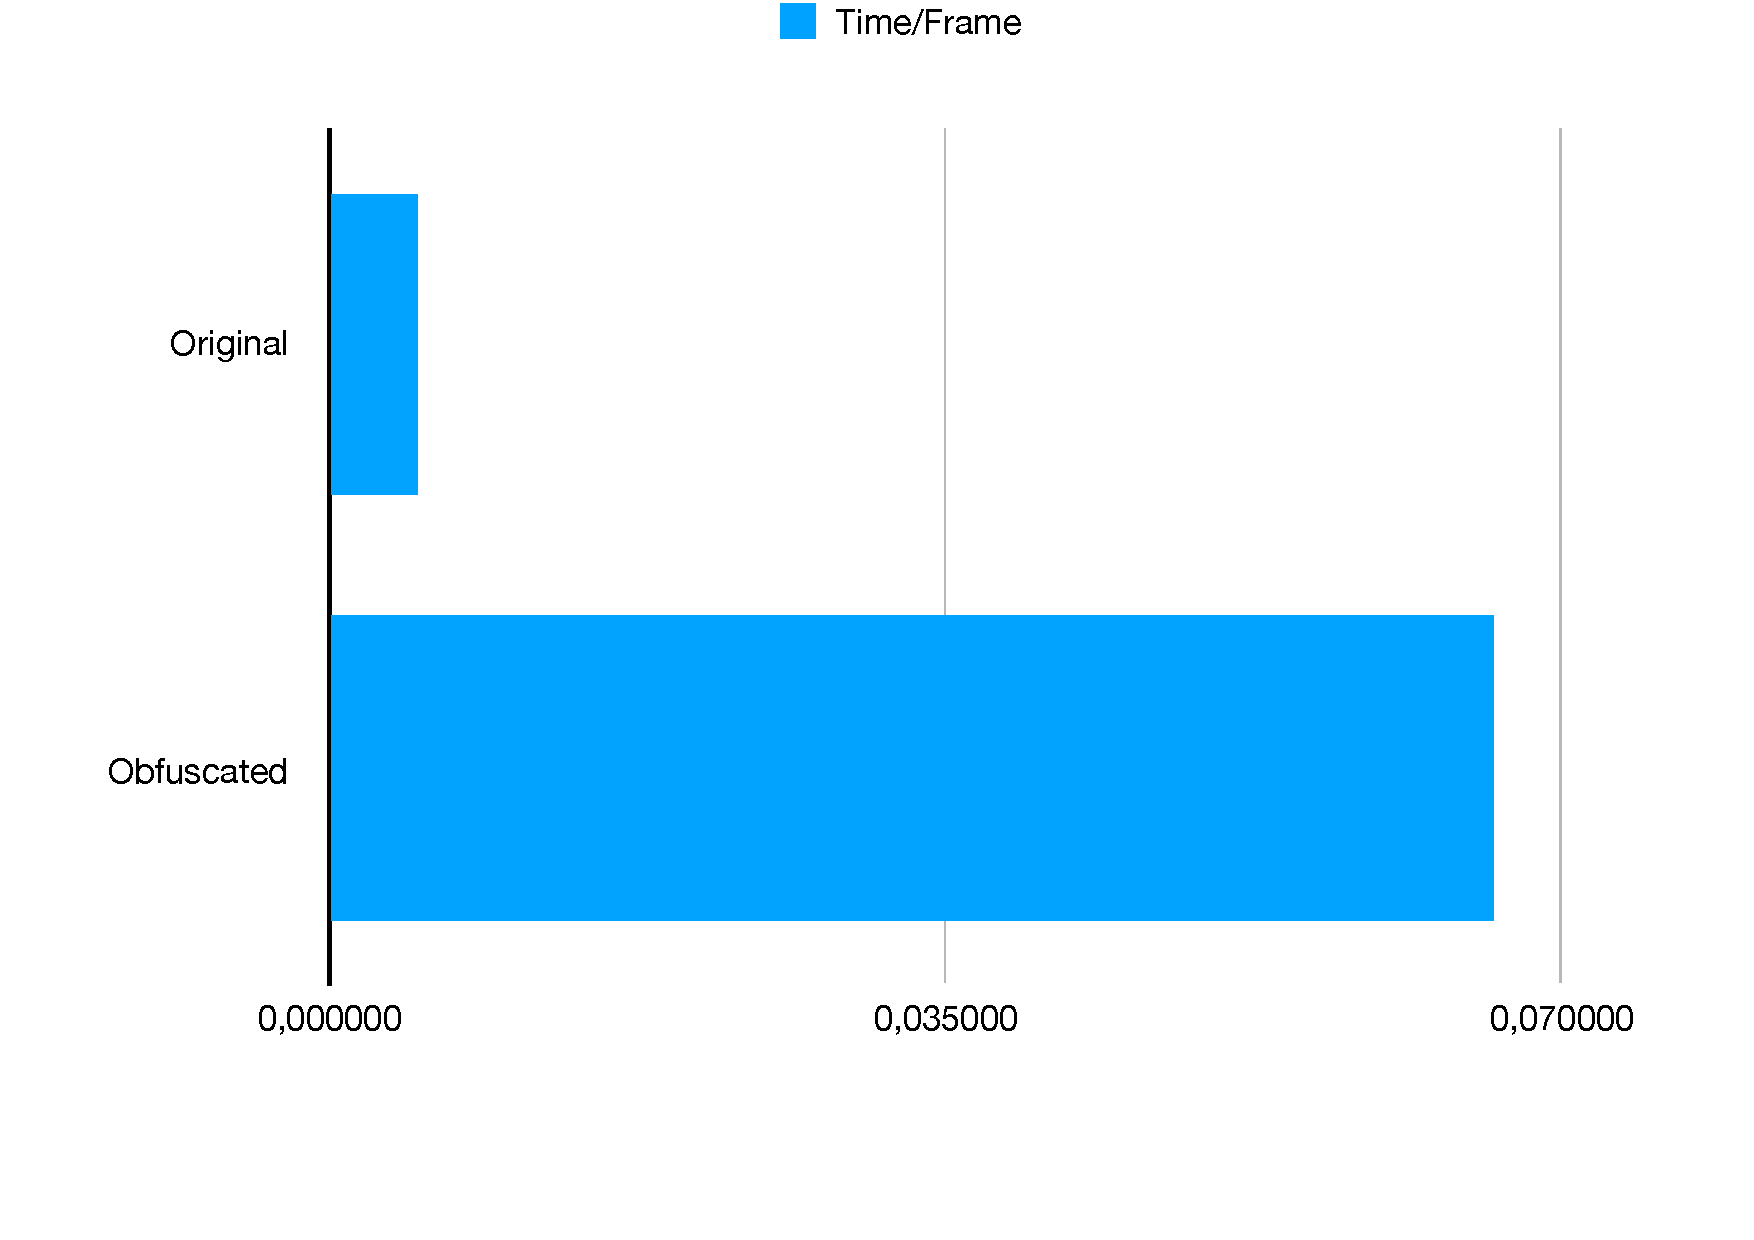
\includegraphics[width=1\textwidth]{./images/bench.pdf}
\caption{Benchmarks}
\end{figure}

Overall the time it took to render a single frame was \textbf{~13,13} times slower then the original program without
obfuscations. The program was executed on an Apple M1 chip.

The program was run via $lli$, without any further optimization passes, which is the LLVM IR code interpreter.

The IR file was generated from compiling the C program, available under the $demo$ folder in the repository with $-emit-llvm$ flag.